% LaTeX Arquivo para Currículos
% Adicione na mesma pasta o arquivo: res.cls

\documentclass{res}

\usepackage[english]{babel}
\usepackage[utf8x]{inputenc}
\usepackage{fancyhdr}  % manter 2 linhas no cabeçalho
\usepackage{graphicx}  % adicionar imagens
\usepackage{url}       % adicionar páginas

\renewcommand{\headrulewidth}{0pt} % suprime a linha do cabeçalho
\setlength{\headsep}{24pt}  % espaço entre o cabeçalho e o texto
\setlength{\headheight}{24pt} % permite a 2a. linha do cabeçalho
\pagestyle{fancy} % estilo da pagina
\rhead{ {\it F. Anselmo}\\{\it page. \thepage} } % cabeçalho da 2a. página
\cfoot{} % rodape vazio
\topmargin=-0.5in % start text higher on the page

\begin{document}
	
	\thispagestyle{empty} % Esta página não possui cabeçalho
	\name{FERNANDO ANSELMO\\[5pt]}
	\address{{\bf Brazil - Brasília} -- Asa Norte \\
		Cel Phone. (+55061) 99874.0763 \\  Phone (+55061) 3201.5834}
	
	\begin{resume}
		
		\section{BRIEFING}
		\vspace{8pt}
		Specialized in Information Technology Management with strong experience in Oracle Database, PostgreSQL, MS SQL Server in addition to NoSQL banks like Hadoop and MongoDB. Knowledge of Java and Python programming and has the analytical skills needed to find the providential needle in the haystack of the data collected by the company. Responsible for the development of dashboards with the ability to analyze data and detect trends, author of 16 books and several articles in specialized magazines, lecturer in several seminars on technology. Focused on learning and bringing changes to the organization with in-depth knowledge of the business.
		
		\section{HABITABILITY}
		\vspace{8pt}
		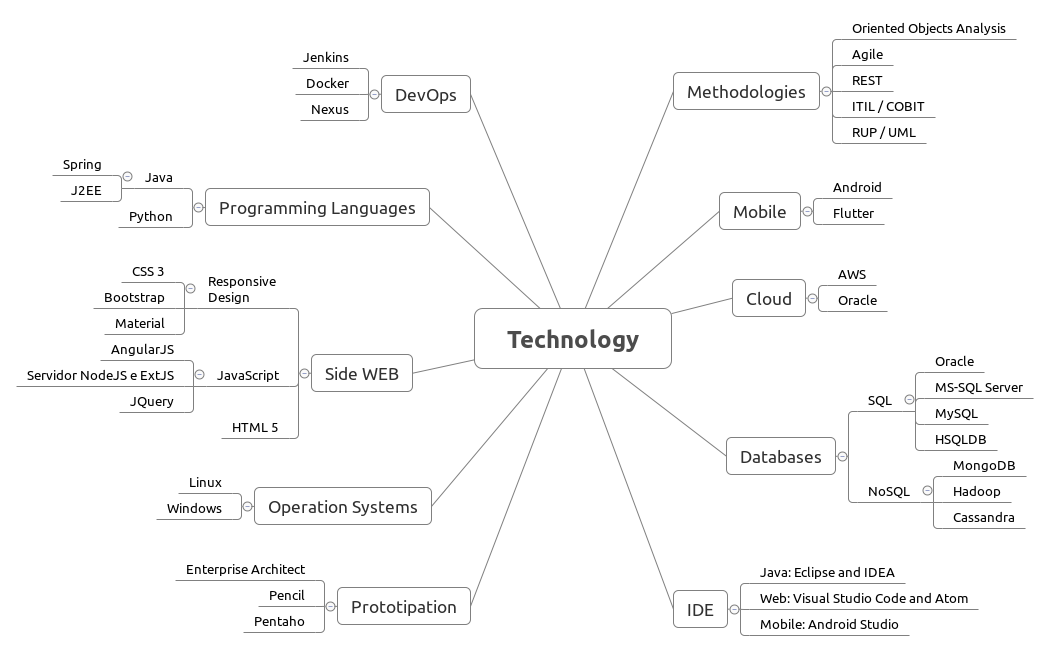
\includegraphics[width=1.0\textwidth]{imagens/technology}
		
		\section{CERTIFICATIONS AND TITLES}
		\vspace{8pt}
		{\sl Java Champion}, Oracle \hfill Dez/2006 \\
		{\sl Sun Certified Programmer for the Java 2 Platform 1.4}, Sun Microsystems \hfill May/2004 \\
		{\sl Java Standard Edition 6 Programmer Certified Professional}, Oracle \hfill Jan/2013 \\
		{\sl Java Enterprise Edition 5 Web Component Developer Certified Professional}, Oracle \hfill Jan/2013 \\
		{\sl Oracle 10g Database Specialist Sales Champion}, Oracle \hfill Jan/2008 \\
		{\sl Oracle 10g Technical sales Champion}, Oracle \hfill Jan/2008 \\
		{\sl Several certificates in official courses SAP, Microsoft, Oracle, Unisys e RCM}
		
		\section{EDUCATION}
		\vspace{8pt} 
		{\sl Specialization}: Católica University | Computer Programming
		\hfill Dez/1996 \\
		{\sl Graduation}: FacSenac University | Information Technology Management
		\hfill Dez/2011 \\
		{\sl Graduate Degree}: JK University | Advanced Business Management 
		\hfill Fev/2016 \\
		{\sl Graduate Degree}: Anhanguera University | Applied Statistics
		\hfill Jan/2020
		
		\section{LANGUAGES} 
		\vspace{18pt}
		\begin{description}
			\item[English] -- Advanced level for both reading and writing.
			\item[Spanish] -- Advanced level for both reading and writing.
		\end{description}
		
		\section{EXPERIENCE IN VOLUNTARY WORK AND CAUSES}
		\vspace{8pt} 
		{\sl DFJUG - Java Users Group} -- Coordinator \hfill Jan/2000 - Actual
		\begin{itemize}
			\item List moderator, assist activities Rybená project (\url{http://www.dfjug.org/rybena.jsp}) 
			which allows the communication via mobile devices between deaf and blind people. Responsible for implementation
			of the JEDI Project in Brazil that aims to teach Java at distance (\url{http://www.dfjug.org/jedi/index.jsp}).
		\end{itemize}
		
		{\sl Magazine Segunda Empregável} -- Editor \hfill Oct/2013 - Oct/2015
		\begin{itemize}
			\item Weekly magazine editor that assists professionals seeking employment in the labor 
			market (\url{http://fernandoanselmo.orgfree.com/wordpress/?page_id=173}).
		\end{itemize}
		
		\section{PROFESSIONAL HISTORY} % Da mais nova para mais antiga
		\vspace{8pt}
		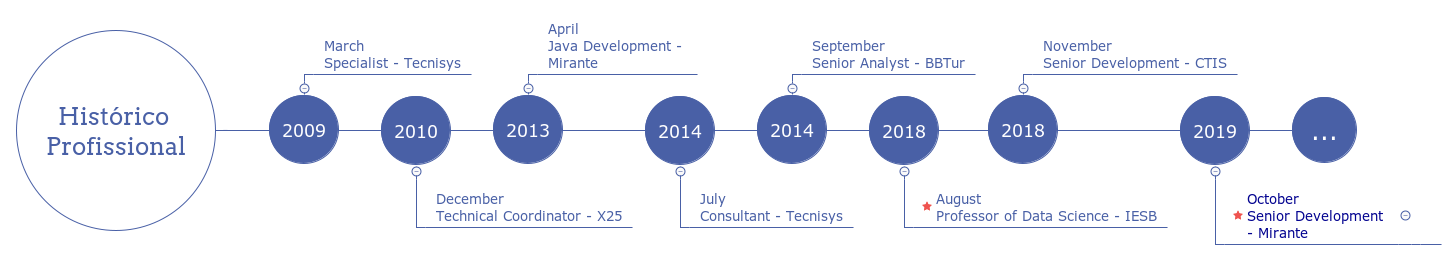
\includegraphics[width=1.0\textwidth]{imagens/experience}
		
		% Mais Recente
		{\sl Mirante Technology} \hfill Oct/2019 - Actual
		\begin{itemize}
			\item Hired to provide software project development services to the customer Bancorbrás. Use of the Spring Boot framework to build Micro Services to serve the company in a Corporate way. Synchronization of the environment with the use of Jenkins / Docker for automation and availability of services. Development in Java technology; Creation of unit tests; Continuous integration and experience in the Oracle Cloud. 
		\end{itemize}
		
		% Mais Recente
		{\sl IESB} \hfill Aug/2018 - Actual
		\begin{itemize}
			\item Hired to act as Professor in the Post graduation in Data Science. With knowledge and skills to use active methodologies in the field of Introduction to Data Science Technologies including knowledge of Python, Hadoop database, Analytical Thinking, Data Quality, Data Mining and Big Data.
		\end{itemize}
		
		{\sl CTIS} \hfill Nov/2018 - Oct/2019
		\begin{itemize}
			\item Responsibilities under the absorption of new systems, for their progress and preparation of documents and environments for "Technology Transfer". Provision of solution to problems and definition of best architectural practices. Technical specification and architecture design of the solutions. Support and definition of technical estimates of demands. Tracking the entire development life cycle and conducting code inspections and developer support. Ensure that the product under development conforms to the defined architecture. I support the technical team in the day-to-day doubts.
		\end{itemize}
		
		{\sl BB Turismo} \hfill Sep/2014 - Nov/2018
		\begin{itemize}
			\item Acted as Senior Systems Analyst and in charge of the maintenance and construction of projects with technology Java, JSF, JQuery, Hibernate in JBoss servers and SQL Server Database. Execution of a Mobile project with the use of PhoneGap, OnsenUI, Angular.js and JQuery technologies. Responsible for organizing all communication of flights and hotels with Amadeus WS / XML through an Ubuntu server with Python for sending and receiving REST / JSON.
		\end{itemize}
		
		{\sl Tecnisys Tecnologias Inovadoras} \hfill Jul/2014 - Aug/2014
		\begin{itemize}
			\item Acted as Consultant in Open Source technologies. Installation and configuration of projects with Jenkis and Nexus, in addition to training with JMeter for testers.
		\end{itemize}
		
		{\sl Mirante Tecnologia} \hfill Apr/2013 - Jun/2014
		\begin{itemize}
			\item Allocated as Senior Java Developer for the Cooperforte client with the objective of perform an Agile project and use Scrum methodology. This project was developed with JSF 2 technology, JQuery, Hibernate in JBoss mirrored servers and use of the MS-SQL Server data. This project had the development carried out in several layers and followed the various standards of proposed projects, such as, Façade, DAO, BO, VO, Factory Method among others.
		\end{itemize}
		
		{\sl X25 Treinamento e Consultoria} \hfill Dec/2010 - Mar/2013
		\begin{itemize}
			\item Survey and development of internal projects to support activities administrative in Java language, using the frameworks Struts2, JSF and database PostgreSQL. Planning and development of training in the Model of Distance Learning. Selection of a solid teacher base (based on experience, certifications, class time, didactic, commitment, among others). Instructor of the courses of Requirements Management, Function Point Analysis, Miscellaneous in the Java Career
			and Android.
		\end{itemize}
		
		{\sl Tecnisys Tecnologias Inovadoras} \hfill Mar/2009 - Nov/2010
		\begin{itemize}
			\item Survey and development of client applications using frameworks JSF and SEAM. Support and aid to the Board of Directors in the construction of administrative and Agility in Project Management. Creation of interactive applications for realization of research on the Web and sending relevant subjects in edicts. Allocated on client for Java / JSP environment migration to the JBoss server. Elaboration of documents of requirements, estimates and detailing requirements with the client.
		\end{itemize}
		
		\section{MORE INFORMATION}
		\vspace{18pt} 
		\begin{description}
			\item[Personal Page] \url{http://fernandoanselmo.orgfree.com/wordpress/}
			\item[Personal Blog] \url{http://fernandoanselmo.blogspot.com/}
			\item[Profile in Linkedin] \url{http://www.linkedin.com/pub/fernando-anselmo/23/236/bb4}
		\end{description}
		
	\end{resume} 
\end{document}